\documentclass[12pt]{article}
\usepackage[utf8]{inputenc}
\usepackage[T2A]{fontenc}
\usepackage[russian]{babel}
\usepackage{amsmath}
\usepackage{amssymb}
\usepackage{dsfont}
\usepackage[dvipsnames]{xcolor}
\usepackage{setspace}
\usepackage{multirow}
\usepackage[a4paper, outer=1.5cm, inner=1.5cm, top=1cm, bottom=1cm]{geometry}
\usepackage{graphicx}
\usepackage{skull}
\usepackage{wasysym}
\usepackage{float}
\graphicspath{{.images/}}
\usepackage{hyperref}
\hypersetup{colorlinks=true, linkcolor=blue, filecolor=magenta, urlcolor=cyan}
\usepackage[firstpage]{draftwatermark}
\SetWatermarkText{
    $\qquad\qquad\qquad\qquad\qquad$\parbox{7cm}{\begin{center}
    
\includegraphics[width = 0.08\textwidth]{lion-logo.png}\bigskip\\~\bigskip\\~\vspace{-24mm}\\~\end{center}}
}
\SetWatermarkAngle{0}
\SetWatermarkScale{1.5}
\usepackage{etoolbox}

\newtoggle{ifsolved}
\newtoggle{needhelp}
\newcounter{num}
\setcounter{num}{1}

\newcommand{\newnum}{\par\textbf{\textnumero\arabic{num}}\stepcounter{num}}
\newcommand{\sol}{\vspace{3mm}\par\textbf{Решение: }}
\newcommand{\ans}{\vspace{3mm}\par\textbf{Ответ: }}
\newcommand{\hint}{\vspace{3mm}\par\textbf{Подсказка: }}
\newcommand{\mode}[1]{
\ifstrequal{#1}{0}{\togglefalse{ifsolved}\togglefalse{needhelp}}{\ifstrequal{#1}{1}{\togglefalse{ifsolved}\toggletrue{needhelp}}{\ifstrequal{#1}{2}{\toggletrue{ifsolved}\togglefalse{needhelp}}{\toggletrue{ifsolved}\toggletrue{needhelp}}}}} %if 0 - if 1 - if 2 - else
%\newenvironment{problem}[8]{%#1, #2, #3
%\parbox{\linewidth}{\vspace{4mm}\ifstrequal{#4}{(лёгкая)}{\newnum\textbf{.}}{\newnum\textbf{*.} } \\ #5}
%\iftoggle{ifsolved}{\sol #6}{}
%\iftoggle{ifsolved}{\ans #7}{}
%\iftoggle{needhelp}{\hint #8}{}}

\newenvironment{problem}[8]{%#1, #2, #3
\parbox{\linewidth}{\vspace{5mm}\ifstrequal{#4}{(лёгкая)}{\newnum\textbf{.}}{\newnum\textbf{*.} } \\ #5}
\iftoggle{ifsolved}{\sol #6}{}

\iftoggle{ifsolved}{\parbox{\linewidth}{\ans #7}}{}
\iftoggle{needhelp}{\parbox{\linewidth}{\hint #8}}{}}

\newenvironment{mylist} %custom list
{ \begin{itemize}
    \setlength{\itemsep}{0pt}
    \setlength{\parskip}{0pt}
    \setlength{\parsep}{0pt}     }
{ \end{itemize}                  }

\newenvironment{homeass}[1]{\vspace*{-1.5cm}
\iftoggle{ifsolved}{
    \section*{\center{Решение домашнего задания к #1.}}
}{
    \section*{\center{\textcolor{Sepia}{Домашнее задание к #1}}}
} \vspace{7mm}\large}

\parindent=0pt
\pagestyle{empty}
%$\!$[\arabic{class}.\arabic{num}]
%\ifnumcomp{\value{counter}}{>}{1}{true}{false}
%\definecolor{Gray}{gray}{0.9}
%\definecolor{mypink}{RGB}{219, 48, 122}
%\newcolumntype{g}{>{\columncolor{Gray}}p{2.8cm}}

\begin{document}
\large
\mode{7}
%0 for problems without hints
%1 for problems + hints
%2 for problems + solutions + answers
%else: show all

{\centering\section*{СПИСОК ЗАДАЧ}}

{\centering\subsection*{\smallskip\\\textcolor{green}{\textbf{Полезные вещи, которые можно и нужно копипастить:}}}}

\subsection*{\textcolor{Emerald}{\textbf{Полезные шпаргалки по LaTeXу:}}}

\textbf{Пример вставки рисунка:}

\begin{minipage}{\linewidth}
    \begin{minipage}{0.54\linewidth}
    см. рисунок справа\\
    Текст к собственно пикче, примерно всегда это либо развёрнутое описание, либо большая часть решения задачи --- стремимся экономить пространство, если это можно сделать.
    \end{minipage}
    \hspace{0.05\linewidth}
    \begin{minipage}{0.4\linewidth}
    \begin{figure}[H] 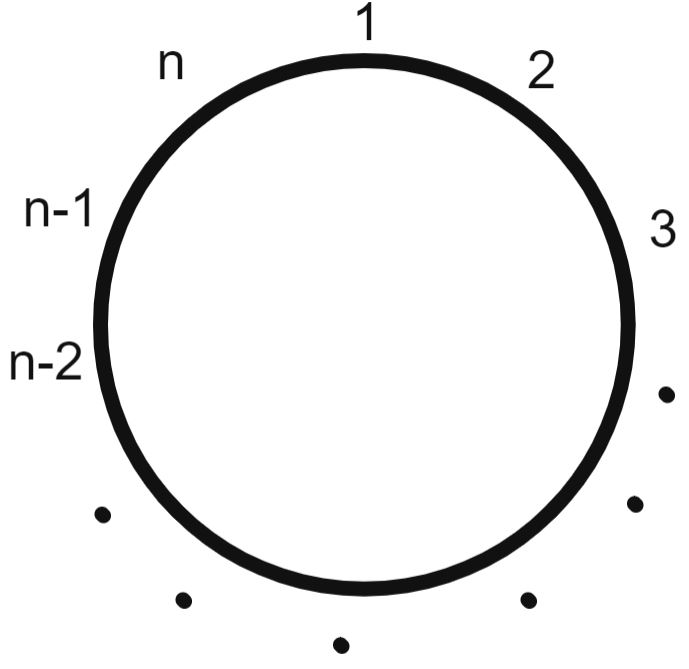
\includegraphics[width=\linewidth]{sol3} %тут поменять имя пикчи
    \end{figure}
    \end{minipage}
\end{minipage}

\textbf{Дефолтные математические знаки и символы:}\\
$\geqslant$,
$\leqslant$,
$a^{b}$,
$x_{i}$,
$\sqrt{a}$,
$\frac{a}{b}$,
$\displaystyle \frac{a}{b}$,
$\cdot$
$\;\Rightarrow\;$,
$\;\Leftrightarrow\;$,
$1{,}2$.
О промежутках:
$a\!b$,
$a\,b$,
$a\:b$,
$a\;b$,
$a\quad b$.

\textbf{Стандартные система и совокупность уравнений / неравенств:}\\
$\left\{
\begin{aligned}
f(x) &= 0 \\
g(x) &= 1
\end{aligned}\right.$

$\left[\begin{aligned}
&\left\{\begin{aligned}
f(x) &\geqslant a \\
g(x) &= b
\end{aligned}\right.\\
&\left\{\begin{aligned}
f(x) &< a \\
g(x) &= -b
\end{aligned}\right.
\end{aligned}\right.$

\subsection*{\textcolor{Emerald}{\textbf{Не математическое, но полезное:}}}
% комментарий в любом месте документа, который нигде не будет видно. Можно использовать для написания заметок-вопросов по задачам
\textbf{Пример таблицы:}

\begin{tabular}{|c|c|c|}
\hline
    $a$ & $b$ & текст
\\\hline
    $c$ & $d$ & мораль
\\\hline
\end{tabular}\\

\textbf{Отступы:} между\smallskip\\ строками\medskip\\ \textbf{Тире} --- это три дефиса.\\
\textbf{Списки:}
\begin{mylist}
\item [$\bullet$] это был пункт а
\item [2)] а это уже пункт номер 2 с изменённым заголовком
\end{mylist}

\subsection*{\textcolor{Emerald}{\textbf{Всё, неупомянутое выше (или если просто что-то не так):}}}
\begin{mylist}
\item [$\bullet$] Решение отдельных вопросов касательно ТеХа нужно искать в \href{https://www.mccme.ru/free-books/llang/newllang.pdf}{Львовском}.

\item [$\bullet$] Найти произвольный символ, который нужен, можно в \href{http://detexify.kirelabs.org/classify.html}{Detexify}.

\item [$\bullet$] Если возникли сомнения при решении, ответ практически ко всем задачам можно проверить с помощью \href{https://www.wolframalpha.com/}{WolframAlpha}.

\item [$\bullet$] Если в задаче нужно создать картинку, то лучше пока отложить эту задачу. Все графики планируется централизованно нарисовать (или перерисовать) в геогебре.

\item [\textcolor{brown}{\textbf{!!}}] Важно ставить \textcolor{red}{\textbf{$\spadesuit$}}
(или просто red) в тело задачи в случае серьёзных вопросов к решению и какой-то вопиющей лажи.

\item [\textcolor{brown}{\textbf{!!}}] Важно ставить \textcolor{olive}{\textbf{$\spadesuit$}}
(или просто olive) в тело задачи в случае не самого удачного текста и кривых отступов.
\end{mylist}

\subsection*{\textcolor{Violet}{\textbf{Комментарии:}}}% а также невидимые комментарии - так можно оставлять заметки-вопросы прямо в задаче, чтобы потом было понятно, в чём вопрос.
\begin{mylist}
\item [$\skull$] Переставлять задачи местами --- очень плохая идея.

\item [$\smiley$] При двойном клике по тексту pdf справа происходит автоматический переход к этому месту в латех-коде, а для обратного перехода можно нажать стрелку вправо (висит сверху между pdf и латех-кодом).

\item [$\smiley$] Если есть размышления, дописывать red/olive к задаче или не дописывать, то лучше всё-таки дописать.

\item [$\skull$] Самое плохое, что можно сделать --- написать в любое поле из трёх (НаписанноеРешение/ВерныйОтвет/Подсказка) только половину того, что надо, никак это не отметить, и потом пойти дальше.\\ Нужно в этот момент писать red/olive в случайном месте задачи, чтобы потом вычислить это с помощью Ctrl+F по всему документу (и это то, что потом будет делаться долго и тщательно)
\end{mylist}

\newpage
\setcounter{num}{901}

\hypertarget{8.5}{{\centering\section*{\bigskip\\\textcolor{Blue}{\hyperlink{start2}{\textcolor{Blue}{8.5}} Комбинаторика, статистика, теория вероятностей-1.}\vspace{-5mm}}}}

\begin{problem}{Комбинаторика. Правило умножения.}{8.5.1}{7A}{(лёгкая)}
{Сколькими способами можно упорядочить Аню, Борю, Витю, и Гену, стоящих на лестнице?}
{НаписанноеРешение}
{ВерныйОтвет}{Подсказка}
\end{problem}

\begin{problem}{Комбинаторика. Правило умножения.}{8.5.1}{6K}{(лёгкая)}
{В футбольной команде $11$ человек, и нужно выбрать капитана и его заместителя.\\ Сколькими способами можно это сделать? (варианты <<А-капитан, Б-заместитель>> и <<Б-капитан, А-заместитель>>, считаются различными вариантами)}
{НаписанноеРешение}
{ВерныйОтвет}{Подсказка}
\end{problem}

\begin{problem}{Комбинаторика. Правило умножения.}{8.5.1}{6K}{*}
{В списке литературы на лето есть $4$ книги. Сколько есть способов выбрать из этих четырёх книжек две, которые будут прочитаны в первую очередь?}
{НаписанноеРешение}
{ВерныйОтвет}{Подсказка}
\end{problem}

\begin{problem}{Комбинаторика. Правило умножения.}{8.5.1}{6K}{(лёгкая)}
{Некто забыл пароль от сейфа, состоящий из $4$ цифр, но помнит, что все цифры различны и среди них есть девятка.\\ Какое максимальное число комбинаций придётся ему набрать, если он пытается открыть сейф, перебирая все возможные варианты?}
{НаписанноеРешение}
{ВерныйОтвет}{Подсказка}
\end{problem}

\begin{problem}{Комбинаторика. Правило умножения.}{8.5.1}{6K \textcolor{red}{\textbf{$\spadesuit$}} \textcolor{olive}{\textbf{$\spadesuit$}}}{*}
{\vspace{-6mm}\\\begin{minipage}{\linewidth}
    \begin{minipage}{0.5\linewidth}

    На рисунке изображены дороги, соединяющие города $A, B, C, D$. Перемещаться можно только по стрелкам. В каком из двух случаев у путника есть больше вариантов маршрутов из $A$ в $D$, и сколько всего путей существует?

    \end{minipage}
    \hspace{0.05\linewidth}
    \begin{minipage}{0.44\linewidth}
        \begin{figure}[H]
        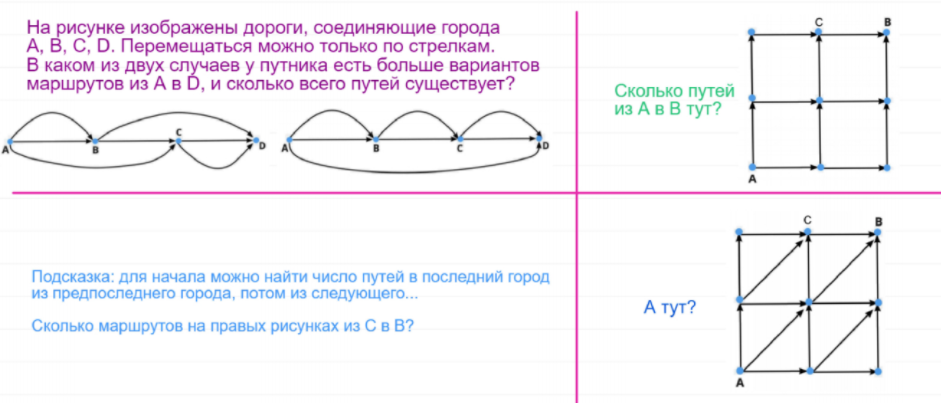
\includegraphics[width=\linewidth]{6K-15}
        \end{figure}
    \end{minipage}
\end{minipage}}
{НаписанноеРешение}
{ВерныйОтвет}{Подсказка}
\end{problem}

\begin{problem}{Комбинаторика. Правило умножения.}{8.5.1}{6K}{(лёгкая)}
{Номер городского телефона в Москве (не считая кода города) состоит из семи цифр, но не может начинаться на 0, например: $129{-}87{-}65$.\\ Сколько всего существует различных телефонных номеров?}
{НаписанноеРешение}
{ВерныйОтвет}{Подсказка}
\end{problem}

\begin{problem}{Комбинаторика. Правило умножения.}{8.5.1}{6K}{(лёгкая)}
{Номер автомобиля состоит из трёх букв русского алфавита (согласно Википедии, используется $12$ букв) и трёх цифр: сначала идёт буква, затем три цифры, а затем ещё две буквы. Сколько существует различных номеров автомобилей?}
{НаписанноеРешение}
{ВерныйОтвет}{Подсказка}
\end{problem}

\begin{problem}{Комбинаторика. Правило умножения.}{8.5.1}{7A}{(лёгкая)}
{На обед можно выбрать один из трёх различных супов, одно из пяти основных блюд, ломтик белого или чёрного хлеба, и на сладкое один из 4 десертов.\\ Сколькими способами может пообедать голодный Алексей, если он никогда и ни за что не ест чёрный хлеб?}
{НаписанноеРешение}
{ВерныйОтвет}{Подсказка}
\end{problem}

\begin{problem}{Комбинаторика. Правило умножения.}{8.5.1}{6K}{(лёгкая)}
{В морозильнике лежат эскимо, фруктовый лёд, шербет и шоколадный стаканчик, на столе лежат клубника, черешня и черника. Также есть напитки: яблочный сок и морс. Сколько можно составить различных десертов, если сразу несколько мороженых включить в один десерт нельзя (может заболеть горло), и в любой десерт должен входить ровно один напиток и одна из ягод?}
{НаписанноеРешение}
{ВерныйОтвет}{Подсказка}
\end{problem}

\begin{problem}{Комбинаторика. Правило умножения.}{8.5.1}{6K}{*}
{Вася и Петя спорят в столовой летнего лагеря: Вася говорит, что Петя не сможет каждый день месяц подряд есть новый набор блюд во время обеда, а Петя считает, что сможет. Во время обеда нужно выбрать один суп (борщ, окрошку, или свекольник), один салат (оливье или греческий), основное блюдо (котлеты с гречкой, запеканка, рыба с картошкой или пельмени со сметаной).\\ Также нужно выбрать напиток (компот или кисель), а десерты в обед не входят и подаются потом, во время полдника.
\\a) Кто выиграет пари?
\\b) Кто выиграл бы пари, если бы в споре речь шла о $2$ месяцах?
\\c) А кто выиграл бы пари, если бы в споре речь бы шла о двух
месяцах, а дело происходило бы не в летнем лагере, а в школе с точно таким же меню?
\\d) Сколько вообще всего рабочих дней в месяце, а сколько~--- в году (если не считать праздники)?}
{НаписанноеРешение}
{ВерныйОтвет}{Подсказка}
\end{problem}

\begin{problem}{Комбинаторика. Правило умножения.}{8.5.1}{6K}{*}
{Злобный хакер пытается подобрать пароль. На проверку $100000$ паролей компьютер хакера тратит $1$ секунду.\\ Сколько (примерно) времени у него уйдёт на то, чтобы:
\\a) Подобрать PIN ($4$ цифры, от $0$ до $9$)? Пример пароля~--- $1234$;
\\b) Подобрать пароль из $6$ символов, каждый символ~--- английская буква $a{-}z$ без учета регистра (то есть всего $26$ вариантов)? Пример~--- abcdfe;
\\c) Подобрать пароль из $6$ символов, каждый символ~--- либо буква $a{-}z$, либо\\ цифра $0{-}9$? Пример пароля~--- ma04cr;
\\d) Подобрать пароль из $8$ символов, каждый символ~--- либо буквы $a{-}z$, либо $A{-}Z$, либо цифры $0{-}9$, либо один из $18$ спецсимволов? Пример~--- Dr5\#t0!l.}
{НаписанноеРешение}
{ВерныйОтвет}{Подсказка}
\end{problem}

\begin{problem}{Комбинаторика. Правило умножения.}{8.5.1}{9D}{(лёгкая)}
{Кубик бросают трижды. Среди всех возможных результатов есть такие, в которых хотя бы один раз встречается шестёрка. Сколько их?}
{НаписанноеРешение}
{ВерныйОтвет}{Подсказка}
\end{problem}

\begin{problem}{Комбинаторика. Правило умножения.}{8.5.1}{7A \textcolor{red}{\textbf{$\spadesuit$}} в число сочетаний}{(лёгкая)}
{Показать, что невозможна такая ситуация, что среди 5 человек у каждого ровно 3 друга (среди этих же 5 человек)}
{НаписанноеРешение}
{ВерныйОтвет}{Подсказка}
\end{problem}

\begin{problem}{Комбинаторика. Правило умножения.}{8.5.1}{6K}{*}
{Сколько можно придумать четырёхзначных чисел, у которых сумма цифр равна $5$, а произведение цифр равно $0$?}
{НаписанноеРешение}
{ВерныйОтвет}{Подсказка}
\end{problem}

\begin{problem}{Статистика.}{8.5.2}{9D}{(лёгкая)}
{Во Вторую мировую войну венгерскому математику Абрахаму Вальду, работавшему в нью-йоркской лаборатории, поручили найти решение важной задачи.\\ Не все американские бомбардировщики возвращались на базу.\\ А на тех, что возвращались, оставалось множество пробоин от зениток и истребителей, но распределены они были неравномерно: больше всего на фюзеляже и крыльях, меньше в топливной системе и намного меньше~--- в двигателе.\\ Значило ли это, что в пробитых местах нужно больше брони? Почему?}
{НаписанноеРешение}
{ВерныйОтвет}{Подсказка}
\end{problem}

\begin{problem}{Статистика.}{8.5.2}{9D}{(лёгкая)}
{Учащиеся 9 класса проходили тестирование по математике, где оценка выставлялась по 100-балльной шкале. Средняя оценка 10 учащихся составила 81 балл. Какой должна быть средняя оценка остальных 20 учащихся класса, чтобы средняя оценка всего класса была 85 баллов?}
{НаписанноеРешение}
{ВерныйОтвет}{Подсказка}
\end{problem}

\begin{problem}{Теория вероятностей.}{8.5.3}{7A}{(лёгкая)}
{Игральный кубик кидают дважды.\\ Каковы шансы того, что в сумме получится 9?}
{НаписанноеРешение}
{ВерныйОтвет}{Подсказка}
\end{problem}

\begin{problem}{Теория вероятностей.}{8.5.3}{9D}{(лёгкая)}
{Билет на электричку стоит 50 рублей, а штраф за безбилетный проезд~--- 450 рублей. Если безбилетник (заяц) попадается контролёру, то оплачивает и штраф, и стоимость билета.\\ Известно, что контролёр встречается в среднем один раз на десять поездок.\\ <<Заяц>> ознакомился с основами теории вероятностей и решил придерживаться стратегии, которая делает математическое ожидание расходов наименьшим.\\
Как ему следует поступать: покупать билет каждый раз, не покупать никогда, или бросать монетку~--- покупать билет или нет?}
{НаписанноеРешение}
{ВерныйОтвет}{Подсказка}
\end{problem}

\begin{problem}{Теория вероятностей.}{8.5.3}{9D}{(лёгкая)}
{Из 5 деталей 3~--- бракованные. Сколько в среднем потребуется проверок, прежде чем обнаружится первая дефектная деталь? (подразумевается, что после проверки деталь откладывается в сторону)}
{НаписанноеРешение}
{ВерныйОтвет}{Подсказка}
\end{problem}

\begin{problem}{Теория вероятностей.}{8.5.3}{9D \textcolor{olive}{\textbf{$\spadesuit$}}}{*}
{\vspace{-6mm}\\\begin{minipage}{\linewidth}
    \begin{minipage}{0.5\linewidth}

    Согласно одной неправдоподобной легенде, Коши и Буняковский очень любили по вечерам играть в дартс. Но мишень у них была необычная~--- сектора на ней были неравные, так что вероятности попасть в разные секторы были не одинаковы. Однажды Коши бросил дротик и попал в мишень. Следующим бросает Буняковский. Что более вероятно: что Буняковский попадёт в тот же сектор, в который попал Коши, или что он попадёт точно в следующий сектор по часовой стрелке?

    \end{minipage}
    \hspace{0.05\linewidth}
    \begin{minipage}{0.44\linewidth}
        \begin{figure}[H]
        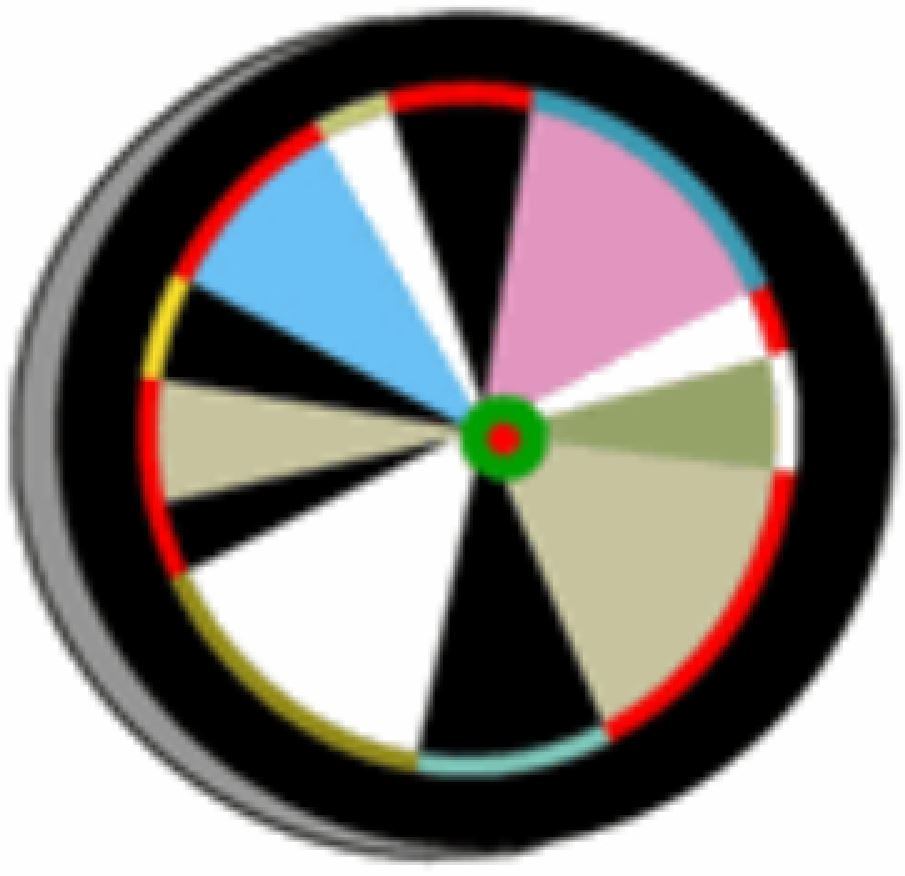
\includegraphics[width=\linewidth]{9D-2}
        \end{figure}
    \end{minipage}
\end{minipage}}
{НаписанноеРешение}
{ВерныйОтвет}{Подсказка}
\end{problem}

\begin{problem}{Теория вероятностей.}{8.5.3}{9D}{(лёгкая)}
{В первой урне находится 7 белых и 3 чёрных шара, во второй урне~--- 8 белых и \\4 чёрных шара, а в третьей урне~--- 2 белых и 13 чёрных.\\ Из этих трёх урн наугад выбирается одна урна. Какова вероятность того, что шар, взятый наугад из этой урны, оказался белым?}
{НаписанноеРешение}
{ВерныйОтвет}{Подсказка}
\end{problem}

\begin{problem}{Теория вероятностей.}{8.5.3}{9D \textcolor{olive}{\textbf{$\spadesuit$}}}{(лёгкая)}
{\vspace{-6mm}\\\begin{minipage}{\linewidth}
    \begin{minipage}{0.5\linewidth}

    В школьном футбольном турнире участвуют 8 команд, одинаково хорошо играющих в футбол. Каждая игра заканчивается победой одной из команд. Случайно выбираемый по жребию номер определяет положение команды в турнирной таблице:\\
    Какова вероятность того, что команды $A$ и $B$:
    \\a) встретятся в полуфинале; \\b) встретятся в финале.

    \end{minipage}
    \hspace{0.05\linewidth}
    \begin{minipage}{0.44\linewidth}
        \begin{figure}[H]
        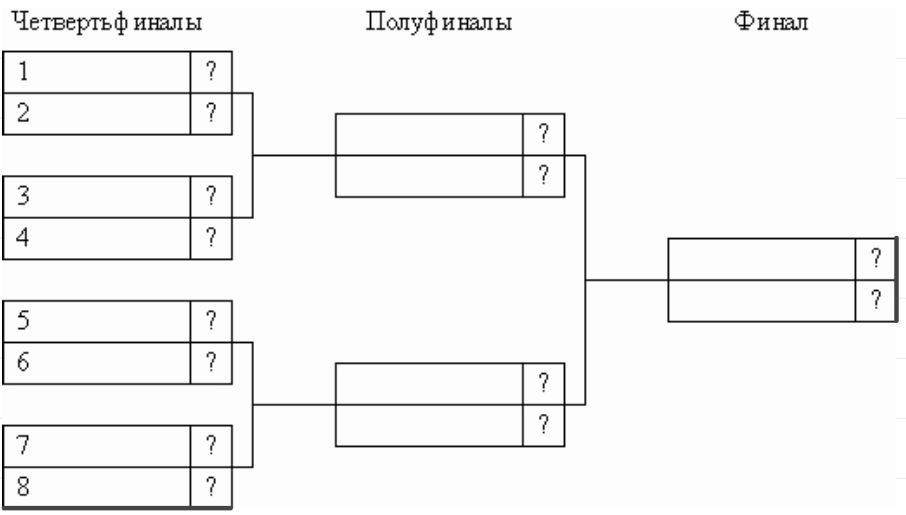
\includegraphics[width=\linewidth]{9D-3}
        \end{figure}
    \end{minipage}
\end{minipage}}
{НаписанноеРешение}
{ВерныйОтвет}{Подсказка}
\end{problem}

\begin{problem}{Теория вероятностей.}{8.5.3}{9D}{*}
{(Покерная задача) Из колоды карт выбирается 5 карт (всего 52 карты без джокеров, достоинством от 2 до туза, всего 13 достоинств, 4 масти, выбор карт случаен).\\ Рассчитать вероятности получения следующих комбинаций:\\
a) Роял-Флэш~--- пять последовательных старших карт одной масти, начиная от туза (туз-К-Д-В-10).
\\b) Стрит-Флэш~--- пять последовательных карт одной масти.
\\c) Каре~--- четыре карты одного достоинства.
\\d) Фулхаус~--- три карты одного достоинства и две другого.
\\e) Флэш~--- все карты одной масти, но не пять идущих подряд.
\\f) Стрит~--- пять последовательных карт, но не все одной масти.
\\g) Тройка~--- три карты одного достоинства (две другие~--- разного).
\\h) Две пары~--- две карты одного достоинства и две другого.
\\i) Пара~--- две карты одного достоинства (но при этом ничего из случаев выше).}
{НаписанноеРешение}
{ВерныйОтвет}{Подсказка}
\end{problem}

\begin{problem}{Теория вероятностей.}{8.5.3}{9D}{(лёгкая)}
{В казино имеется рулетка, которая с вероятностью по $\frac{1}{2}$ выпадает на чёрное и на красное. Игрок, поставивший сумму $n$ и угадавший цвет, получает обратно сумму $2n$ (а если не угадывает цвет, то теряет всю сумму).\\ Вася играет по следующей схеме: сначала он ставит доллар. Если он выигрывает, то покидает казино, а если проигрывает, то удваивает ставку и ставит два доллара. Если выигрывает, то покидает казино, а если проигрывает, то снова удваивает ставку и ставит четыре доллара, и так далее, пока не выиграет в первый раз или у него не хватит денег на новую удвоенную ставку.\\ У Васи до входа в казино имеется 1050 долларов.\\
a) Какова вероятность того, что Вася покинет казино после выигрыша?
\\b) Каков ожидаемый выигрыш (математическое ожидание) Васи?}
{НаписанноеРешение}
{ВерныйОтвет}{Подсказка}
\end{problem}

\begin{problem}{Теория вероятностей.}{8.5.3}{9D}{(лёгкая)}
{В жюри из трёх человек два члена независимо друг от друга принимают правильное решение с вероятностью $p$, а третий для вынесения решения кидает монетку (окончательное решение выносится большинством голосов). Жюри из одного человека выносит справедливое решение с вероятностью $p$.\\ Какое из этих жюри чаще выносит справедливые решения?}
{НаписанноеРешение}
{ВерныйОтвет}{Подсказка}
\end{problem}

\begin{problem}{Теория вероятностей.}{8.5.3}{9D}{(лёгкая)}
{Пятеро человек купили билеты в кино~--- 5 мест в одном ряду подряд. Среди этих 5 человек есть Алиса и Александр, которые хотели бы сидеть рядом, и Борис и Белла, которые хотели бы того же. Хильде же всё равно где сидеть.\\ Из 5 билетов, полученных на кассе, каждый случайным образом вытащил один. Какова вероятность, что:
\\a) Никому не нужно будет меняться билетами между собой (все и так довольны)?
\\b) Кому-то надо будет поменяться билетами, так как ни в паре А, ни в паре Б люди не сидят рядом друг с другом?
\\c) Одна пара довольна своими билетами, а другая пара~--- нет?}
{НаписанноеРешение}
{ВерныйОтвет}{Подсказка}
\end{problem}

\begin{problem}{Теория вероятностей.}{8.5.3}{9D}{(лёгкая)}
{В коробке 123 чёрных шара и 321 белый шар. Наугад извлекается пара шаров.\\
Если оба шара одного цвета, то вместо пары в коробку кладётся белый шар. Если же извлечённая пара шаров разного цвета, то вместо неё кладётся чёрный шар. Так повторяется до тех пор, пока в корзине не останется один шар. \\Какова вероятность того, что этот шар будет чёрным?}
{НаписанноеРешение}
{ВерныйОтвет}{Подсказка}
\end{problem}

\begin{problem}{Теория вероятностей.}{8.5.3}{9D}{(лёгкая)}
{В классе 30 учеников. Показать, что вероятность того, что у каких-нибудь двух учеников совпадают дни рождения, составляет больше $\frac{1}{2}$.\\ (в предположении, что вероятность дня рождения в определённый день равна $\frac{1}{365}$)

}
{НаписанноеРешение}
{ВерныйОтвет}{Подсказка}
\end{problem}

\begin{problem}{Теория вероятностей.}{8.5.3}{9D}{(лёгкая)}
{В произвольном выпуклом шестиугольнике независимо друг от друга выбраны две различные случайные диагонали. Найти вероятность того, что эти диагонали пересекаются внутри шестиугольника (внутри~--- значит не в вершине)}
{НаписанноеРешение}
{ВерныйОтвет}{Подсказка}
\end{problem}

\begin{problem}{Теория вероятностей.}{8.5.3}{9D}{(лёгкая)}
{Чтобы сбить самолёт, достаточно одного попадания. По самолёту было сделано три выстрела~--- с вероятностями попадания $0{,}1$, $0{,}2$ и $0{,}4$ соответственно.\\ Какова вероятность того, что самолёт был сбит?}
{НаписанноеРешение}
{ВерныйОтвет}{Подсказка}
\end{problem}

\begin{problem}{Теория вероятностей.}{8.5.3}{9D red непрерывная вероятность, мб 11 класс}{*}
{Двое договорились встретиться в фиксированном месте, но не успели договориться о времени.\\ В результате известно, что каждый из них придёт в промежутке времени от 12:00 до 13:00, но из-за того, что оба не очень терпеливы, известно, что каждый будет ждать только 10 минут~--- то есть, если они придут в 12:34 и 12:43 они встретятся, а если в 12:30 и 12:45~--- нет.\\ Какова вероятность того, что встреча всё же состоится?}
{НаписанноеРешение}
{ВерныйОтвет}{Подсказка}
\end{problem}

\begin{problem}{Теория вероятностей.}{8.5.3}{9D}{(лёгкая)}
{Симметричную (честную) монетку кинули 4 раза.
\\a) Какова вероятность того, что выпало четыре решки?
\\b) Какова вероятность того, что выпало три орла?
\\c) Какова вероятность того, что орлов и решек будет поровну?
\\d) Какова вероятность того, что орлов будет больше, чем решек?
\\e) Какова вероятность того, что модуль разности числа орлов и числа решек $|x - y|$ будет равен 2?
\\f) Играли двое, вначале монетку два раза кинул первый, потом два раза кинул второй. Какова вероятность того, что орлов в первых двух бросках столько же, сколько и в последних двух бросках?}
{НаписанноеРешение}
{ВерныйОтвет}{Подсказка}
\end{problem}

\begin{problem}{Теория вероятностей.}{8.5.3}{9D}{(лёгкая)}
{Три усталых ковбоя зашли в салун и повесили свои шляпы на бизоний рог при входе. Когда глубокой ночью ковбои уходили, они уже были не в состоянии отличить одну шляпу от другой и поэтому разобрали три шляпы наугад.\\ Найти вероятность того, что никто из них не взял свою собственную шляпу.}
{НаписанноеРешение}
{ВерныйОтвет}{Подсказка}
\end{problem}

\begin{problem}{Теория вероятностей.}{8.5.3}{9D \textcolor{olive}{\textbf{$\spadesuit$}}}{(лёгкая)}
{\vspace{-6mm}\\\begin{minipage}{\linewidth}
    \begin{minipage}{0.5\linewidth}

    Вася написал на листке бумаги записку, сложил её вчетверо и надписал сверху <<Маме>> (см. фото). Затем он развернул записку, дописал ещё кое-что, опять сложил записку по линиям сгиба случайным образом (не обязательно как раньше) и оставил на столе, положив случайной стороной вверх. Найти вероятность того, что надпись <<Маме>> по-прежнему сверху.

    \end{minipage}
    \hspace{0.05\linewidth}
    \begin{minipage}{0.44\linewidth}
        \begin{figure}[H]
        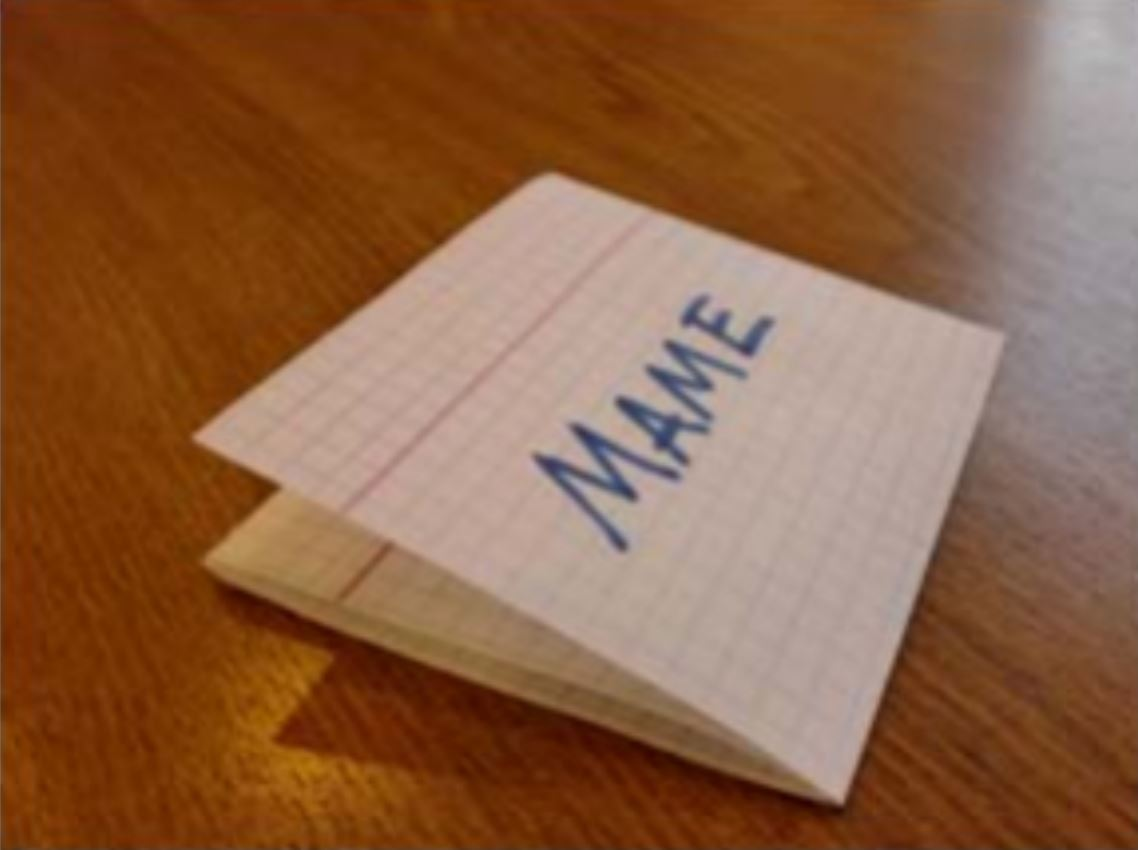
\includegraphics[width=\linewidth]{9D-5}
        \end{figure}
    \end{minipage}
\end{minipage}}
{НаписанноеРешение}
{ВерныйОтвет}{Подсказка}
\end{problem}

\begin{problem}{Теория вероятностей.}{8.5.3}{9D}{(лёгкая)}
{Аня и Боря стреляют в тире. У них есть только один шестизарядный револьвер с одним патроном (на большее денег им не хватило). Поэтому они договорились по очереди крутить барабан и стрелять. Начинает Аня.\\ Найти вероятность того, что выстрел произойдёт, когда револьвер будет у Ани.}
{НаписанноеРешение}
{ВерныйОтвет}{Подсказка}
\end{problem}

\begin{problem}{Теория вероятностей.}{8.5.3}{9D red сложность задачи - нерешаемая за любое время. МБ надо в отдельный список}{*}
{Условие задачи следующее: в тюрьме находится 100 заключенных, каждый из которых имеет личный номер от 1 до 100. Тюремщик решает дать заключенным шанс на освобождение и предлагает пройти придуманное им испытание.\\ Он идёт в секретную комнату и подготавливает 100 коробок с крышками.\\ На каждую коробку он наносит числа с нумерацией от 1 до 100. Затем он приносит 100 бумажных табличек, по числу заключенных, и нумерует эти таблички от 1 до 100. После этого он случайно перемешивает 100 табличек и помещает в каждую коробку по одной табличке, закрывая крышку.\\ Заключенные не видят, как тюремщик выполняет все эти действия.\\
Испытание устроено так: тюремщик отводит каждого заключённого по очереди в комнату с коробками и говорит, что он должен найти коробку, в которой будет находиться табличка с его номером. Заключенные пытаются найти табличку со своим номером, открывая коробки. Каждому разрешается открыть до 50-ти коробок; если КАЖДЫЙ из заключенных найдёт свой номер, то ВСЕХ заключенных отпустят, если же ХОТЯ БЫ ОДИН из них не найдёт свой номер за 50 попыток, то ВСЕ заключенные останутся в тюрьме.\\
Менять местами таблички, оставлять подсказки после начала испытания нельзя, но заключенные перед началом испытания могут собраться вместе и обсудить свою стратегию.\smallskip
\begin{itemize}
    \item [a)] Какова примерно вероятность успеха, если у заключенных не будет никакой стратегии (все открывают случайные коробки)?
    \item [b)] Придумать стратегию, которая хоть немного повышает шансы заключенных на успех.
    \item [c)] Есть СУЩЕСТВЕННО более эффективная стратегия c вероятностью успеха, приблизительно равной \textbf{$0{,}3$ (успех в 30\% случаев)}.\\ Задача~--- попытаться придумать эту стратегию.
\end{itemize}
Для вычислений в этой задаче можно (и нужно) использовать \textcolor{CornflowerBlue}{\href{https://www.wolframalpha.com}{\textbf{WolframAlpha}}}}
{НаписанноеРешение}
{ВерныйОтвет}{Супер-стратегия из пункта с) в определённых случаях не срабатывает.
Но оказывается, что если в самом начале испытания поменять местами две определённые бумажки с номерами, шансы успеха данной стратегии станут равными \textbf{100\% ! !}}
\end{problem}

\begin{problem}{Перестановки, число размещений и сочетаний. Разбиения.}{8.5.4}{9D}{(лёгкая)}
{Сколькими способами можно поставить 8 ладей на шахматную доску так, чтобы они не били друг друга?}
{НаписанноеРешение}
{ВерныйОтвет}{Подсказка}
\end{problem}

\begin{problem}{Перестановки, число размещений и сочетаний. Разбиения.}{8.5.4}{7A}{(лёгкая)}
{Сколькими способами можно выбрать пару из 5 предметов?}
{НаписанноеРешение}
{ВерныйОтвет}{Подсказка}
\end{problem}

\begin{problem}{Перестановки, число размещений и сочетаний. Разбиения.}{8.5.4}{7A}{(лёгкая)}
{На электростанции 22 столба, и каждый соединён проводом с любым другим. Сколько всего проводов на этой электростанции?}
{НаписанноеРешение}
{ВерныйОтвет}{Подсказка}
\end{problem}

\begin{problem}{Перестановки, число размещений и сочетаний. Разбиения.}{8.5.4}{6K}{(лёгкая)}
{Сколько есть способов усадить $7$ человек на $6$ табуреток (кто-то один останется стоять, то есть на одну табуретку садится только один человек)?}
{НаписанноеРешение}
{ВерныйОтвет}{Подсказка}
\end{problem}

\begin{problem}{Перестановки, число размещений и сочетаний. Разбиения.}{8.5.4}{6K}{(лёгкая)}
{Из $9$ ребят собирается команда из трёх человек.\\ Сколько возможных команд может получиться?}
{НаписанноеРешение}
{ВерныйОтвет}{Подсказка}
\end{problem}

\begin{problem}{Перестановки, число размещений и сочетаний. Разбиения.}{8.5.4}{9D}{(лёгкая)}
{Сколько есть способов составить из 8 человек две команды для игры в футбол по 4 человека каждая?}
{НаписанноеРешение}
{ВерныйОтвет}{Подсказка}
\end{problem}

\begin{problem}{Перестановки, число размещений и сочетаний. Разбиения.}{8.5.4}{9D}{(лёгкая)}
{Из двух математиков и десяти экономистов надо составить комиссию из восьми человек. Сколькими способами это может быть сделано, если в комиссии должен быть хотя бы один математик?}
{НаписанноеРешение}
{ВерныйОтвет}{Подсказка}
\end{problem}

\begin{problem}{Перестановки, число размещений и сочетаний. Разбиения.}{8.5.4}{9D}{(лёгкая)}
{Найти число способов разложить число 5 в сумму нескольких произвольных натуральных чисел.}
{НаписанноеРешение}
{ВерныйОтвет}{Подсказка}
\end{problem}

\begin{problem}{Перестановки, число размещений и сочетаний. Разбиения.}{8.5.4}{9I}{(лёгкая)}
{Сколько существует треугольников (не вырождающихся в отрезок) с периметром 18 см, если длина каждой стороны треугольника~--- целое число?}
{НаписанноеРешение}
{ВерныйОтвет}{Подсказка}
\end{problem}

\begin{problem}{Перестановки, число размещений и сочетаний. Разбиения.}{8.5.4}{9D}{(лёгкая)}
{Трое хотят поделить пиццу (8 кусков) и спорят, сколько кусков пиццы и кому должно достаться. В итоге, после долгих споров, они сошлись лишь на том, что каждый из них должен получить хотя бы по одному кусочку пиццы. Сколько есть способов разделить пиццу между ними?\\
(Каждый должен получить целое число кусков, пример решения: $8 = 1 + 3 + 4$)}
{НаписанноеРешение}
{ВерныйОтвет}{Подсказка}
\end{problem}

\begin{problem}{Перестановки, число размещений и сочетаний. Разбиения.}{8.5.4}{9I}{*}
{На мероприятии 10 человек едят пиццу (20 идентичных кусков). Кто-то мог не успеть попробовать, кто-то другой мог съесть любое целое количество кусков (хоть все 20). Сколько есть различных способов разделения пиццы между всеми участниками мероприятия?\\
(Каждый должен получить целое число кусков, пример : $20 = 20 + \underbrace{0 + \ldots 0}_{\text{9 нулей}}$)}
{НаписанноеРешение}
{ВерныйОтвет}{Подсказка}
\end{problem}

\begin{problem}{Бином Ньютона.}{8.5.5}{7A}{(лёгкая)}
{Если выписать треугольник Паскаля и вычеркнуть единички по краям, то все числа во второй строке делятся на 2, в третьей строке~--- на 3, но в четвёртой, однако, на 4 не делятся. В каких ещё строках выполнено это свойство? Доказать.

}
{НаписанноеРешение}
{ВерныйОтвет}{Подсказка}
\end{problem}

\begin{problem}{Бином Ньютона.}{8.5.5}{9D}{(лёгкая)}
{У человека есть 10 друзей и в течение нескольких дней он приглашает некоторых из них в гости так, чтобы компания ни разу в точности не повторялась (в какой-то из дней он может не приглашать никого).\\ Сколько дней подряд он сможет так делать?}
{НаписанноеРешение}
{ВерныйОтвет}{Подсказка}
\end{problem}

\begin{problem}{Бином Ньютона.}{8.5.5}{9D \textcolor{red}{\textbf{$\spadesuit$}} \textcolor{olive}{\textbf{$\spadesuit$}}}{(лёгкая)}
{\vspace{-6mm}\\\begin{minipage}{\linewidth}
    \begin{minipage}{0.5\linewidth}

    Найти число способов пройти от перекрёстка $A$ до перекрёстка $B$ (см. рисунок), если перемещаться можно только по прямым улицам, и двигаться можно только вниз и вправо.

    \end{minipage}
    \hspace{0.05\linewidth}
    \begin{minipage}{0.44\linewidth}
        \begin{figure}[H]
        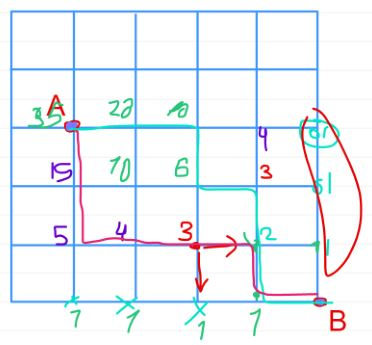
\includegraphics[width=\linewidth]{9D-4}
        \end{figure}
    \end{minipage}
\end{minipage}}
{НаписанноеРешение}
{ВерныйОтвет}{Подсказка}
\end{problem}

\begin{problem}{Бином Ньютона.}{8.5.5}{6K}{(лёгкая)}
{Убедиться, что сумма всех чисел в $8$ строчке треугольника Паскаля $(1$, $8, \ldots)$ равна $256 = 2*2*2*2*2*2*2*2$ (восемь двоек).}
{НаписанноеРешение}
{ВерныйОтвет}{Подсказка}
\end{problem}

\begin{problem}{Бином Ньютона.}{8.5.5}{6K \textcolor{olive}{\textbf{$\spadesuit$}}}{(лёгкая)}
{\vspace{-6mm}\\\begin{minipage}{\linewidth}
    \begin{minipage}{0.5\linewidth}

    Заполнить в треугольнике Паскаля ещё $3$ строки.

    \end{minipage}
    \hspace{0.05\linewidth}
    \begin{minipage}{0.44\linewidth}
        \begin{figure}[H]
        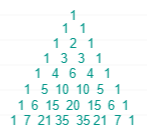
\includegraphics[width=\linewidth]{6K-13}
        \end{figure}
    \end{minipage}
\end{minipage}}
{НаписанноеРешение}
{ВерныйОтвет}{Подсказка}
\end{problem}

\begin{problem}{Условная вероятность.}{8.5.6}{9D}{(лёгкая)}
{Кубик кинули дважды, и вычислили сумму полученных очков.\\ Какова вероятность того, что на каком-то кубике выпала шестёрка, если известно, что эта сумма оказалась равна \\a) 7 \hfill b) 10 \hfill c) 9}
{НаписанноеРешение}
{ВерныйОтвет}{Подсказка}
\end{problem}

\begin{problem}{Условная вероятность.}{8.5.6}{9D}{(лёгкая)}
{В первой урне находится 7 белых и 3 чёрных шара, во второй урне~--- 8 белых и 4 чёрных шара, а в третьей урне~--- 2 белых и 13 чёрных.\\ Из этих трёх урн наугад выбирается одна урна. Какова вероятность того, что была выбрана первая урна, если шар, взятый наугад из этой урны, окажется белым?}
{НаписанноеРешение}
{ВерныйОтвет}{Подсказка}
\end{problem}

\begin{problem}{Условная вероятность.}{8.5.6}{9D}{(лёгкая)}
{Среди определённой группы людей вероятность некоторой болезни равна $0{,}02$. Тест, позволяющий выявить болезнь, несовершенен. На больном он даёт верный результат в 98 случаях из 100, а на здоровых пациентах в 4 случаях из 100 даёт ошибочный результат (указывает на наличие болезни при её отсутствии)\\
Найти вероятность того, что человек, тест которого указывает на наличие болезни, и в самом деле болен.}
{НаписанноеРешение}
{ВерныйОтвет}{Подсказка}
\end{problem}

\begin{problem}{Условная вероятность.}{8.5.6}{9D}{(лёгкая)}
{Кубик кидают 3 раза. Известно, что сумма очков на всех кубиках равна 7.\\ Какова вероятность того, что ни на одном из кубиков не выпала единица?}
{НаписанноеРешение}
{ВерныйОтвет}{Подсказка}
\end{problem}

\begin{problem}{Условная вероятность.}{8.5.6}{9D}{*}
{Кубик кидают 3 раза. Известно, что сумма очков на всех кубиках равна 10. Какова вероятность того, что ни на одном из кубиков не выпало единицы? Двойки?}
{НаписанноеРешение}
{ВерныйОтвет}{Подсказка}
\end{problem}

\begin{problem}{Условная вероятность.}{8.5.6}{9D}{(лёгкая)}
{К юбилею монетный двор отчеканил три юбилейные монеты. Одна монета получилась правильно, у второй монеты на обеих сторонах оказался орёл, а у третьей обе стороны~--- решки. Директор монетного двора не глядя выбрал одну из этих трёх монет и наудачу её бросил. Выпал орёл.\\ Чему равна вероятность того, что и на второй стороне этой монеты тоже орёл?}
{НаписанноеРешение}
{ВерныйОтвет}{Подсказка}
\end{problem}

\begin{problem}{Условная вероятность.}{8.5.6}{9D}{(лёгкая)}
{В одной группе из 25 студентов 3 человека имеют высокий уровень подготовки, 19 человек~--- средний и 3~--- низкий. Вероятности успешной сдачи экзамена для данных студентов соответственно равны: $0{,}95$; $0{,}7$ и $0{,}4$.\\ Известно, что некоторый студент экзамен сдал. Какова вероятность того, что:
\\a) он был подготовлен очень хорошо;
\\b) он был подготовлен средне;
\\c) он был подготовлен плохо.}
{НаписанноеРешение}
{ВерныйОтвет}{Подсказка}
\end{problem}

\begin{problem}{Условная вероятность.}{8.5.6}{9D}{*}
{Есть 4 кубика. На трёх из них окрашена белым половина граней, а на четвёртом~--- всего одна. Наудачу выбранный кубик подбрасывается семь раз, в результате чего из этих семи подбрасываний белая грань выпала лишь один раз.\\ Найти вероятность того, что был выбран четвёртый кубик.}
{НаписанноеРешение}
{ВерныйОтвет}{Подсказка}
\end{problem}

\begin{problem}{Условная вероятность.}{8.5.6}{9D}{*}
{Будем говорить, что событие $A$ благоприятствует (способствует) событию $B$, если $\mathbb{P}(B|A) > \mathbb{P}(B)$ (то есть c наступлением события $A$ шансы наступления события $B$ возрастают).\\
Известно, что $A$ благоприятствует $B$, а $B$, в свою очередь, благоприятствует $C$.\\ Верно ли, что $A$ благоприятствует $C$? Придумать пример/контрпример.}
{НаписанноеРешение}
{ВерныйОтвет}{Подсказка}
\end{problem}

\begin{problem}{Условная вероятность.}{8.5.6}{9D}{(лёгкая)}
{На охоте два охотника одновременно и независимо по одному разу каждый выстрелили в кабана. В итоге кабан оказался убит, и в нём была обнаружена ровно одна пуля, однако, поскольку охотники пользуются одинаковыми охотничьими ружьями, нельзя определить, кто именно убил кабана.\\ Охотники хорошо знают, что первый охотник попадает в цель в 8 случаях из 10 ($p = 0{,}8$), а второй~--- в 4 случаях из 10 ($p = 0{,}4$). Найти вероятность того, что:
\\ a) кабана убил первый охотник \hfill и \hfill b) кабана убил второй охотник.}
{НаписанноеРешение}
{ВерныйОтвет}{Подсказка}
\end{problem}

\end{document}